\documentclass[a4paper,10pt]{article}
\usepackage[utf8]{inputenc}
\usepackage{amsmath}
\usepackage{mathrsfs}
\usepackage{amsfonts}
\usepackage{mathtools}  
\usepackage{graphicx}
\usepackage{authblk}
\usepackage[final]{pdfpages}
\usepackage[a4paper, total={6in, 9in}]{geometry}
\mathtoolsset{showonlyrefs}  

%\DeclareMathOperator*{\argmax}{argmax} % thin space, limits underneath in displays
\DeclareMathOperator*{\argmax}{arg\,max} % Jan Hlavacek
\setlength{\parindent}{0cm}

%opening
\title{Problem Sheet \# 02 (2D Image Processing)}
%\author[1]{Muhammad Shoaib Ahmed Siddiqui (Matrikulation \# 407485)}
%\author[2]{Muhammad Jameel Nawaz Malik (Matrikulation \# 400382)}
\author[1]{Muhammad Shoaib Ahmed Siddiqui (Matrikulation \# 407485) \\ Muhammad Jameel Nawaz Malik (Matrikulation \# 400382)}

\begin{document}

\maketitle

% Problem # 01
\section{}

\subsection{}
What is “hysteresis” in image edge detection?

\textbf{\underline{Solution:}} 

"Hysteresis" is a thresholdor in a Canny operator which suppresses the problem of fragmented edges by using two different thresholds.
The edges whose magnitude lies over the high threshold are definite edges while the edges whose magnitude lies below the low threshold are not edges. The edges whose magnitude lies in between the two thresholds are considered as edges if there are strong edges in between the weak edges.
This helps to ensure that weak edges are not broken up into multiple edge fragments.

\subsection{}
What is the difference between classification and regression?

\textbf{\underline{Solution:}} 

In machine/deep learning, predicting a discrete class among predefined set of classes is called as "Classification". On the other hand, predicting a real-valued continuous output is called as "Regression".

\subsection{}
What is the difference between 'Score function' and 'Loss function'?

\textbf{\underline{Solution:}} 

A score function indicates the sensitivity of the likelihood function $\mathcal{L}(X; \theta)$ w.r.t. to its parameter $\theta$. Loss function on the other hand, serves as a measure for the analysis of a classifier's predictions.
The score function is used to update the parameters of the network in some machine learning algorithms when the likelihood is being computed by the model.

\subsection{}
What is gradient of a function?

\textbf{\underline{Solution:}} 

Gradient is a generalization of the derivative for multi-dimensional cases. It is the rate of change of a function w.r.t. its parameters. It's the slope of the tangent line to the point in the space. It’s a vector (a direction to move) that;
\begin{itemize}
\item Points in the direction of greatest increase of a function.
\item Is zero at a maximum or minimum since the tangent is flat.
\end{itemize}

\subsection{}
Find the gradient of the function $f(x, y, z) = (2 \times x) + (y \times z)$ using back propagation when the input is $x = 1, y = 2, z = 3$.

\textbf{\underline{Solution:}} 

Let $s=y \times z$, and $t=2 \times x$.

\begin{equation}
f(x, y, z) = s + t
\end{equation}

It is evident from the above equation that:

\begin{equation}
\frac{\partial f}{\partial s} = 1
\end{equation}

\begin{equation}
\frac{\partial f}{\partial t} = 1
\end{equation}

Similarly:

\begin{equation}
\frac{\partial s}{\partial z} = y
\end{equation}

\begin{equation}
\frac{\partial s}{\partial y} = z
\end{equation}

\begin{equation}
\frac{\partial t}{\partial x} = 2
\end{equation}

Using the chain rule, the partial derivatives w.r.t. $x, y, z$ can be written as:

\begin{equation}
\frac{\partial f}{\partial x} = \frac{\partial f}{\partial t} \frac{\partial t}{\partial x} = 1 \times 2 = 2
\end{equation}

\begin{equation}
\frac{\partial f}{\partial y} = \frac{\partial f}{\partial s} \frac{\partial s}{\partial y} = 1 \times z = 3
\end{equation}

\begin{equation}
\frac{\partial f}{\partial z} = \frac{\partial f}{\partial s} \frac{\partial s}{\partial z} = 1 \times y = 2
\end{equation}

\subsection{}
What is the use of activation functions in multilayered fully connected networks?

\textbf{\underline{Solution:}} 

Matrix multiplication and convolutions are linear operations. Stacking multiple layers of these operations is again a linear operation i.e. it can be replaced by a single operation. 
In order to take advantage of this hierachy, non-linearity is introduced in the form of the activation functions. The commonly used activation functions are ReLU, sigmoid, and hyperbolic tangent.

\subsection{}
What is the output of the activation volume from a convolutional layer when the input volume is of size 227 x 227 x 3, with the following conv parameters - number of filters: 96, special extent (kernel size): 11x11, stride: 4, padding: 0

\textbf{\underline{Solution:}} 

\begin{align}
H' =& \frac{H - F + 2P}{S} + 1 \\
W' =& \frac{W - F + 2P}{S} + 1
\end{align}

Where $H, W$ are the height and width of the input while $H', W'$ are the height and width of the output, $P$ indicates the amount of zero padding and $S$ denotes the stride.

Given input dimension: $227 \times 227 \times 3$

\begin{align}
H' =& \frac{227 - 11 + 0}{4} + 1 = 55 \\
W' =& \frac{227 - 11 + 0}{4} + 1 = 55
\end{align}

Hence, the output dimension is: $55 \times 55 \times 96$

\section{}
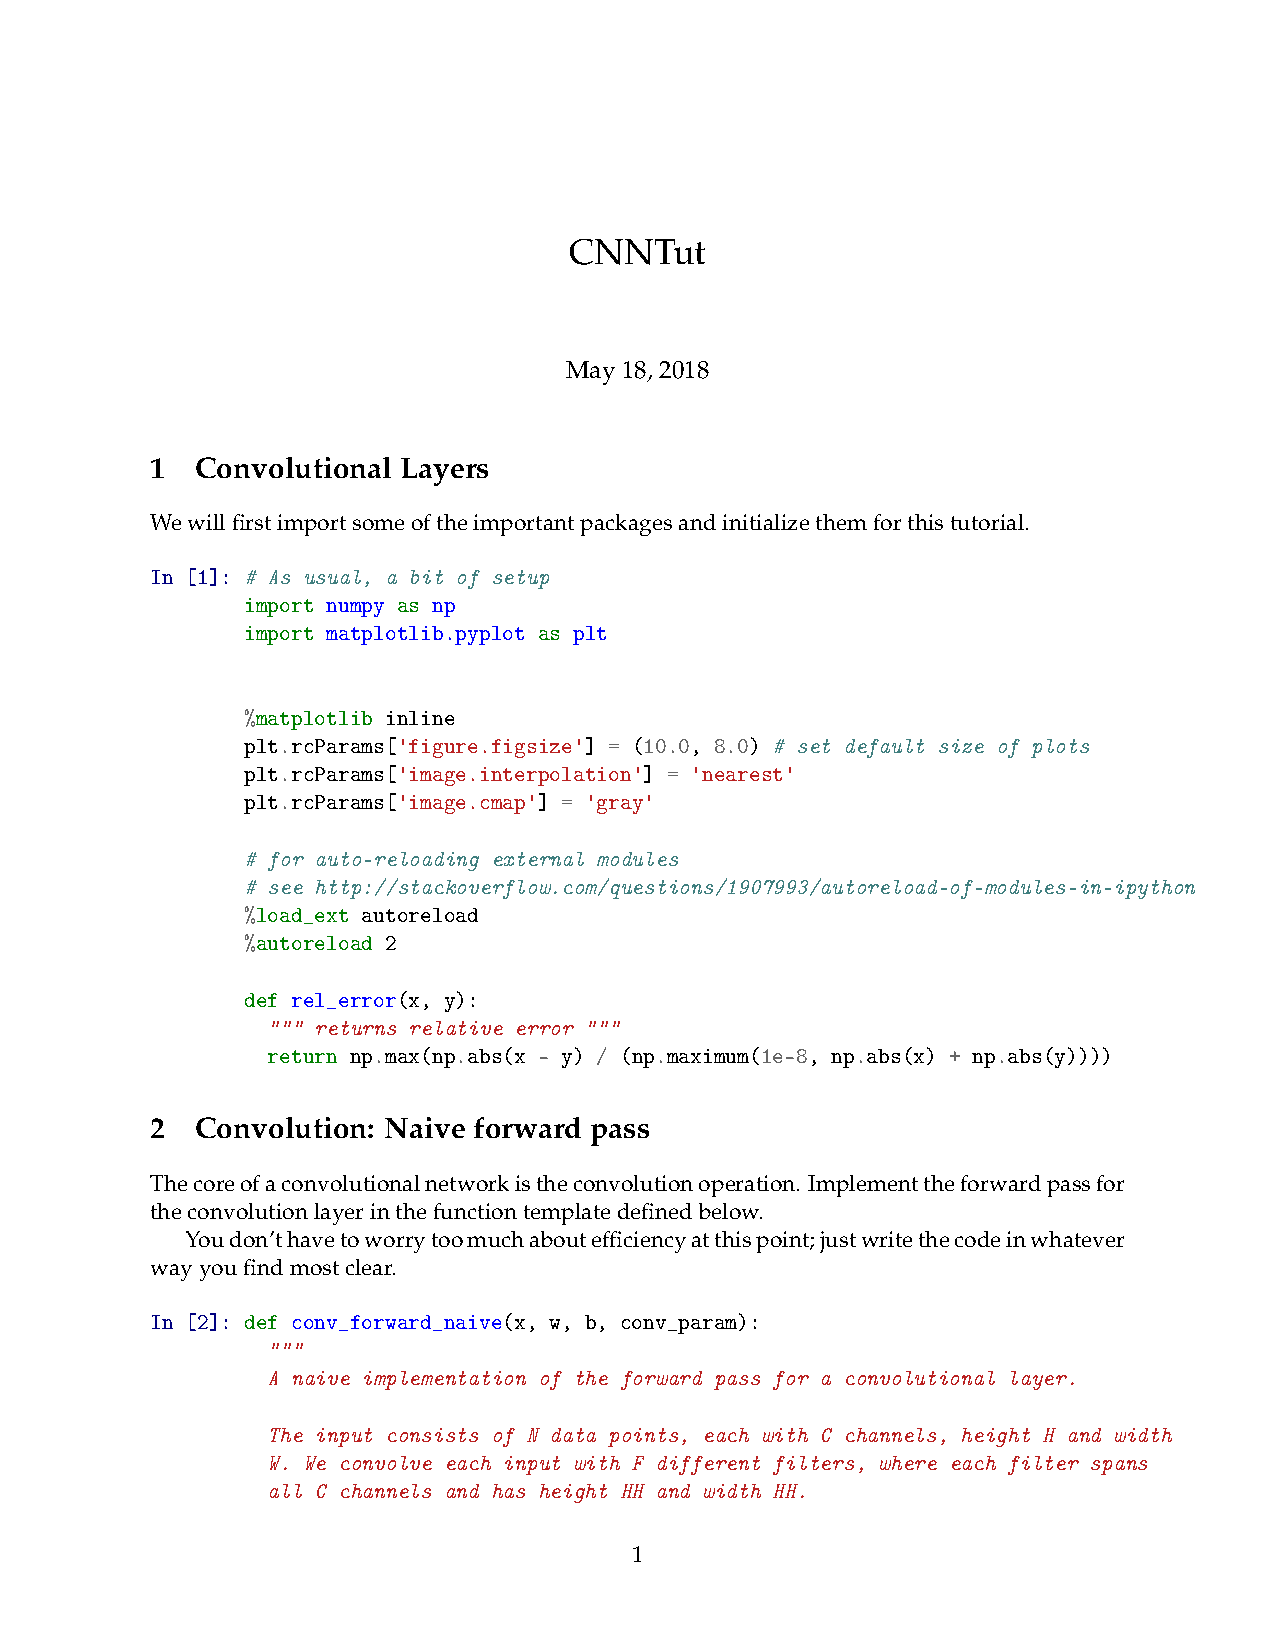
\includepdf[pages=-,pagecommand={},width=\textwidth]{CNNTut.pdf}

\section{}
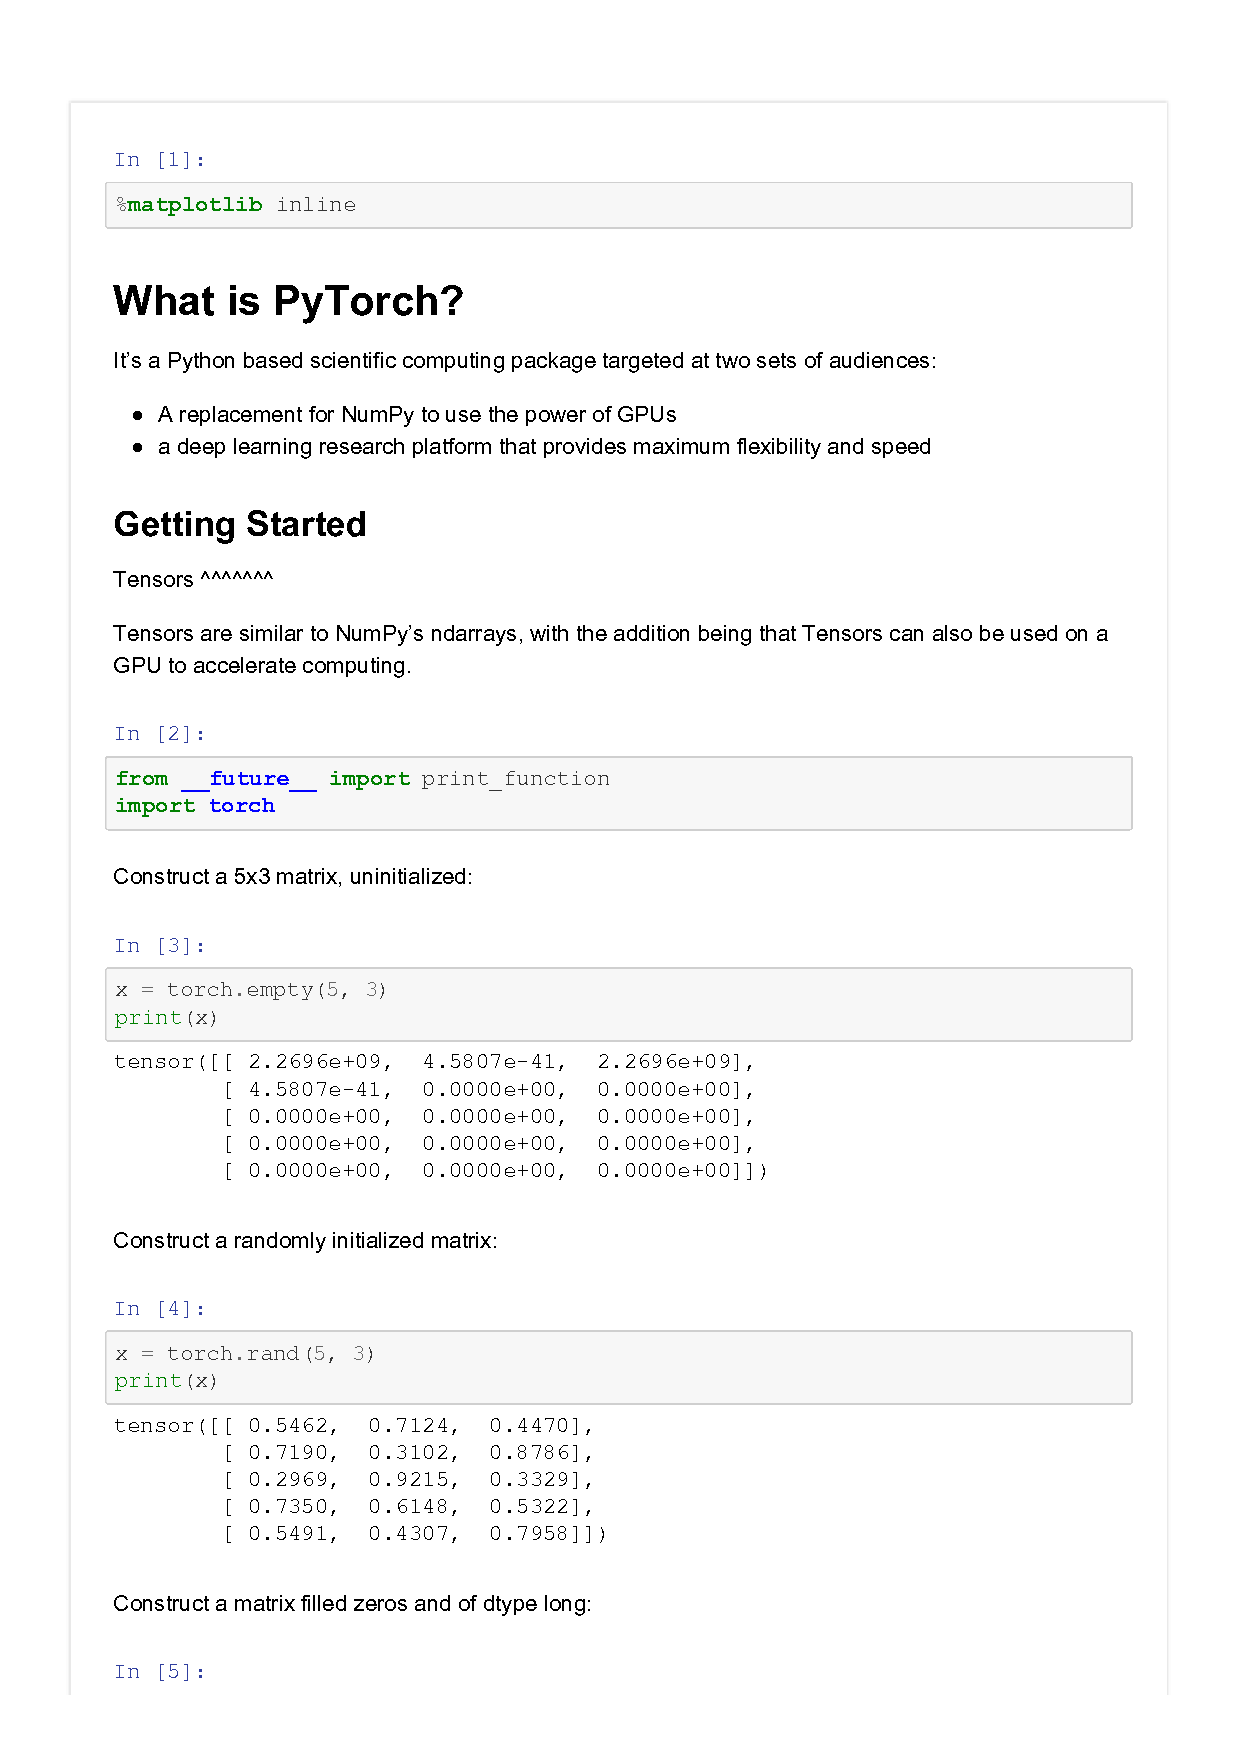
\includepdf[pages=-,pagecommand={},width=\textwidth]{Pytorch-Blitz.pdf}

\end{document}
